\documentclass{ctexart}
\usepackage{enumerate}
\usepackage[colorlinks,linkcolor=blue]{hyperref}

\usepackage{ulem} 
\usepackage{caption}
\usepackage{graphicx}
\usepackage{subfigure}
\newcommand{\pic}[2]{\begin{figure}[h]
\centering
 \includegraphics[width=1.0\textwidth]{#1}
 \caption{#2}
\end{figure}}

\title{霓虹歌姬企画}
\author{南方科技大学日语社}
\begin{document}
\maketitle
\tableofcontents

\section{前言}
前几天日语社的同学们一起去会展中心的伊势海老这个店吃日料,本来想着要不然跟服务员光说日语吧,看看会发生什么事。但是到了店里却觉得店员应该还是不可能懂日语的,遂作罢。我觉得如果想要日语炸店的话,还是要去些人均1000以上的店。虽说店员们不会说日语,可是店里依然飘荡着日语歌。几首歌听下来,觉得还挺好听的,就是我对这些歌曲和歌手都没有什么了解。同学们指出这是某某有名的歌手唱的有名的歌,我才猛然发现我虽然平素也是主要听日本的歌曲,但是对于ACG之外的日本歌曲其实并没有太多的了解。之前社里一起看红白歌会,回忆起廖同学讲着讲那讲得头头是道,加上我有点歌荒,不禁觉得是时候扩展一下我的听歌范围了。之前的我连安室奈美惠都不知道,多亏廖同学指点才算是知道了这么个人名。听歌就像看论文一样,看得多了写个综述是很好的。综述这种东西既有利于自己总结,也便于跟别人分享。遂决定组织各位写这么一个小小的综述集子,来看看日本到底有多少值得注意的歌手。每个词条大概有一张图片,再配上编写者的一些说明,最后给新人一个听歌的顺序,使得新人可以循序渐进地了解与习惯这个歌手的风格。歌手按虚拟偶像,声优,ACG歌手和非ACG歌手分类,方便读者检索。\\
“霓虹歌姬企画”这个名字是我拍脑袋定的。之所以叫歌姬是因为觉得这样叫比较萌。总之就是这样一个集子,感谢各位的贡献。——张子健


\section{虚拟偶像}
\subsection{$\mu$'s}
\begin{figure}[h]
\centering
 
\includegraphics[width=1.0\textwidth]{lovelive.jpg}
 \caption{LoveLive!}
\end{figure}
$\mu$'s是LoveLive!企划里校园偶像组合的名字。“为了拯救濒临废校的学校,九位少女决定组成校园偶像”。我觉得校园偶像这个设定还是很好玩的。我刚入学的时候曾经想要为了\sout{跟妹子玩耍}宣传南科大,在学校里组织一个校园偶像团体。可是实在是找不到合适的妹子,遂作罢。\\
与同一类型的偶像大师相比,虽说LoveLive!的动画做得显然没有偶像大师765要好,但是歌还是很好听的。我个人认为LoveLive!的音乐更胜一筹。其音乐人藤泽庆昌也是少女歌剧和宝石之国的音乐人。\\
LoveLive!的乐趣还在于丰富的真人生放送节目。LoveLive!实际上是一个2.5次元企划,因为虚拟偶像背后的声优本身在企划中也有很多的亮相机会。尤其是当动画本身做得不好的时候,真人节目就变得尤为重要。各位还可以在听了一定量的歌曲之后去找$\mu$'s的演唱会看看。粉丝们的热情与小姐姐们卖力的表演可以感动任何一个有偶像之魂的人。(小姐姐一词据说就是先从LoveLive!的粉丝圈子里面流行起来的)
\subsubsection*{歌曲推荐}
实际上$\mu$'s的曲风还是比较多变的。在这里列出一些笔者喜欢的歌。其中soldier game每次去KTV都想唱...
\begin{enumerate}
\item Angelic Angel
\item No brand girls
\item soldier game
\item 春情ロマンティック
\item Music S.T.A.R.T!!
\end{enumerate}

\subsection{Aqours}
\subsubsection*{歌曲推荐}
\begin{enumerate}
\item 少女以上の恋がしたい
\item 夜空はなんでも知ってるの?
\item 待ってて愛のうた
\item ユメ語るよりユメ歌おう
\end{enumerate}


\subsection{偶像大师 本家}
\begin{figure}[h]
\centering
 
\includegraphics[width=1.0\textwidth]{im@s.jpg}
 \caption{idol m@ster (有没有DitF的感觉?)}
\end{figure}
作为一个本来可以靠粉丝向吃饭的偶像大师本家,硬是做出了无论是谁都可以欣赏的优秀动画。笔者先看的职场番之顶点——SHIROBAKO(白箱)之后才去看的本家动画,虽然说本家动画很难说比白箱好,但是目前笔者还没有看到可以称之为第三名的职场动画。本家动画节奏舒适,铺垫、煽情均十分到位。相比Lovelive系列的动画,本家动画渲染的职场的紧张氛围更让人有真实感,而不是一群女高中生过家家。不过你也不用担心这动画太过紧张刺激。实际上,偶像大师本家动画比白箱好的一个地方就是它更加地欢乐。这种欢乐是跟星际牛仔里的欢乐很像(See 第8集和第9集),笔者甚至认为两者有直接地借鉴关系。

\subsubsection*{歌曲推荐}
\begin{enumerate}
\item M@STERPIECE
\item “HELLO!!”
\item 虹のデスティネーション
\item LEMONADE
\end{enumerate}



\subsection{偶像大师 百万现场}
\subsubsection*{歌曲推荐}
\begin{enumerate}
\item Legend Girl!!
\item Blue Symphony
\end{enumerate}

\subsection{偶像大师 灰姑娘}

\subsection{Poppin'Party}


\subsection{XX:me(キス·ミー)}
\begin{figure}[h]
\centering
 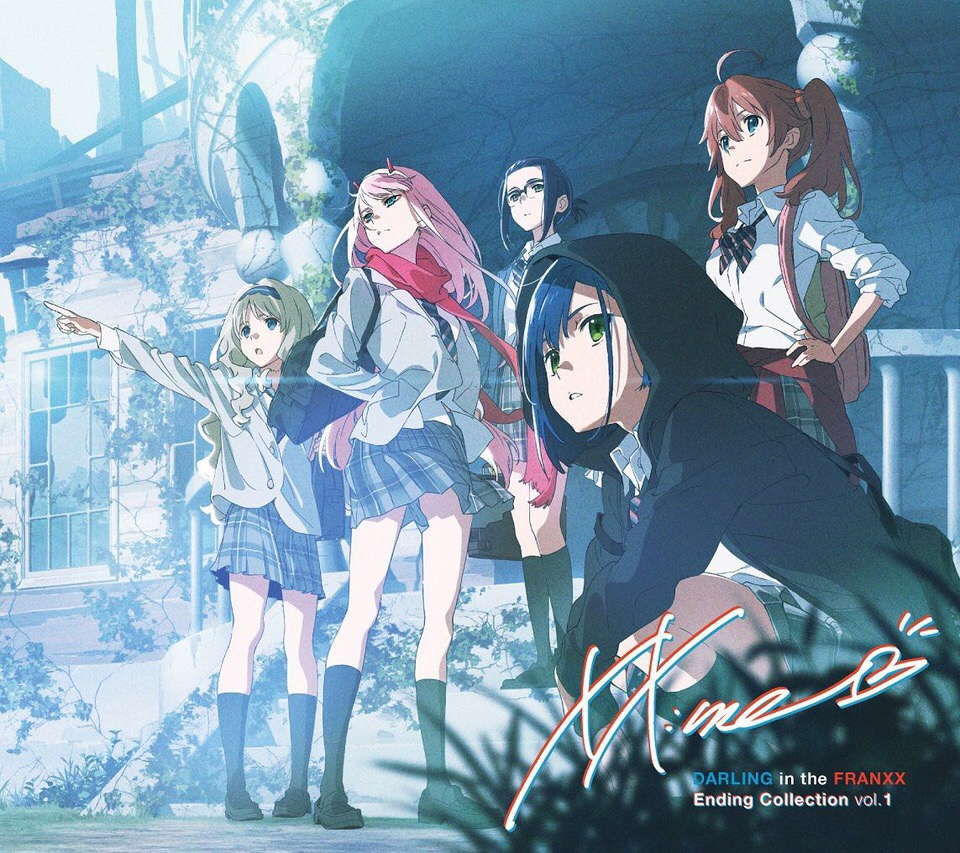
\includegraphics[width=0.7\textwidth]{xx_me.jpg}
 \caption{XX:me}
\end{figure}
XX:me是为了演唱DARLING in the FRANXX(\sout{国家队}DitF)的角色的声优为了演唱动画里的歌曲而形成的临时组合,所以歌曲并不多并且不会增加(除非太阳从西边出来这片子出第二季)
\begin{enumerate}
\item  戸松遥(ゼロツー) 
\item  市ノ瀬加那(イチゴ)
\item  山下七海(ミク)
\item  早見沙織(ココロ)
\item  石上静香(イクノ)
\end{enumerate}

笔者当时追完了DitF动画,看最后几集的时候心情就像被喂了某种东西一样,遂下定决心此番一生黑。可惜这片前半段的表现和人物塑造还是成功的,于是角色们的印象在笔者脑内实在是不能消散。有一天找EVA剧场版的ED-《Beautiful World》的时候猛然发现原来DitF也有一首歌叫这个名字。没想到一听便沦陷,我本以为我已经把这片忘了,结果听到这歌,痛恨制作组使片子烂尾、心疼角色的心情遍迸发出来(导演锦织老贼你给我出来)。笔者认为,DitF的几首ED质量颇高,结合剧情和歌词食用更佳(DitF请务必只看一半)。

\subsubsection*{歌曲推荐}
\begin{enumerate}
\item Beautiful World
\item トリカゴ
\end{enumerate}

\section{专职歌手}
\subsection{Aimer}

\begin{figure}[h]
\centering
 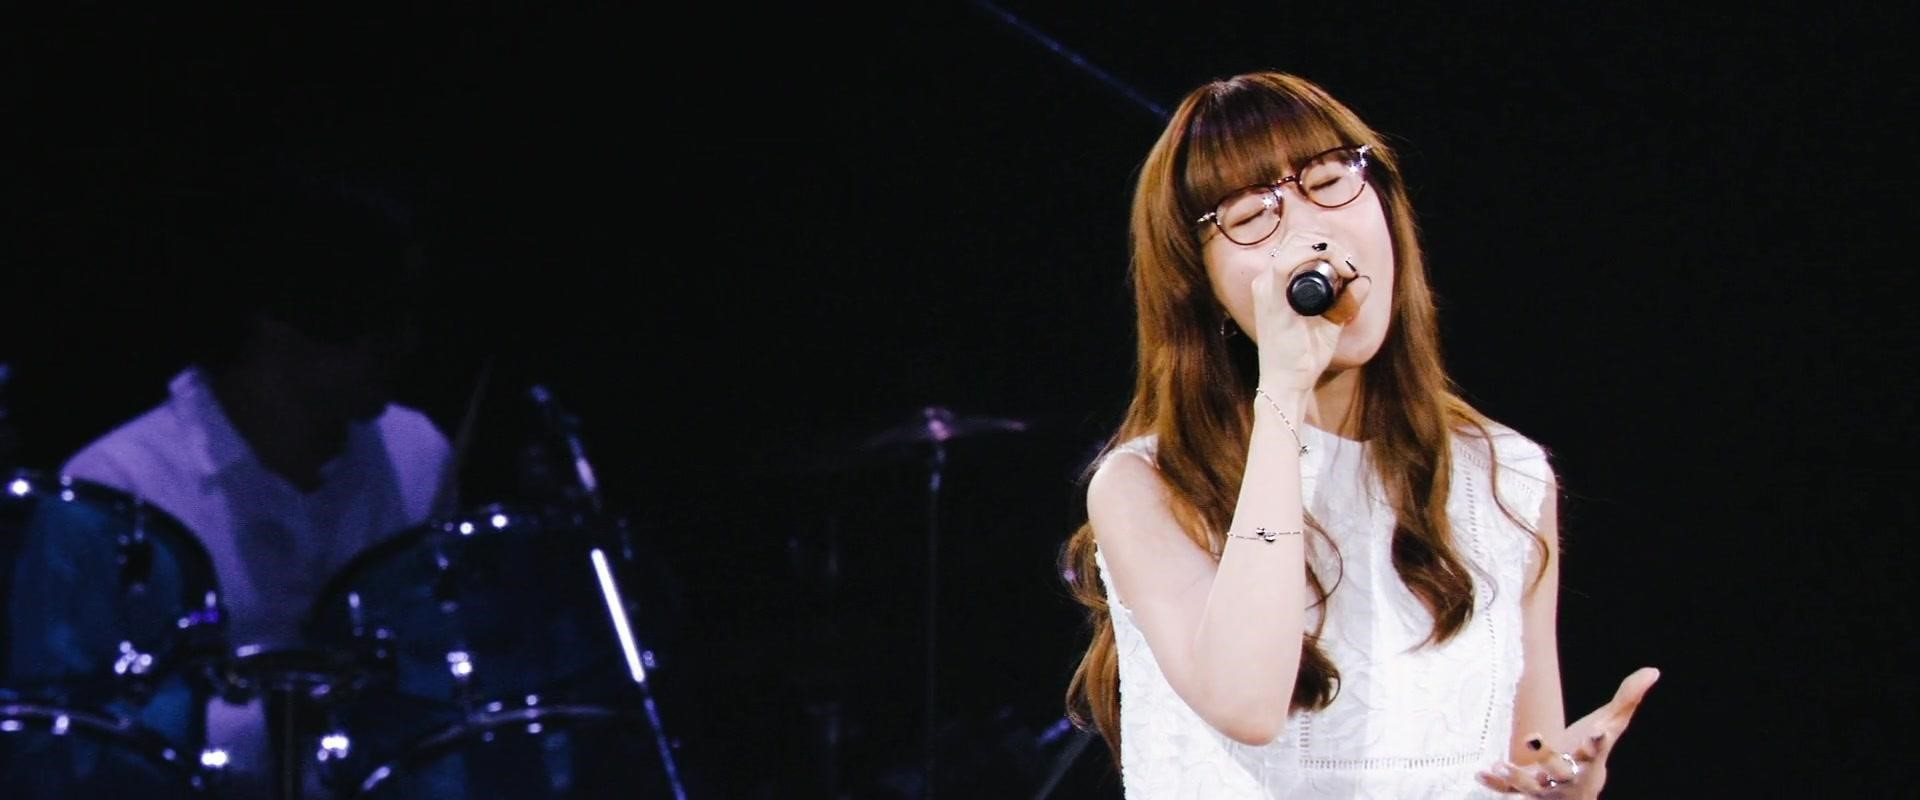
\includegraphics[width=1.0\textwidth]{Aimer.jpg}
 \caption{Aimer}
\end{figure}

想了很久,还是把Aimer放在了第一位。所谓第一位,其所指就是在笔者眼中,作为一位歌姬,Aimer的存在就其音乐上的魅力是无可比拟的。\\
Aimer15岁时喉部病变,一度难以说话。但因祸得福,随着嗓音的逐渐变化,Aimer开发出了一种极为独特的声线,一种令人难以自拔乐不思蜀抚掌击节余音绕梁的声线。孔子有“三月不识肉味”的赞美,我想也不过如此。\\
当然Aimer如今的成就离不开制作人agehasprings的提携。一单《六等星之夜》便一炮而红,她优雅而纯净,略有沧桑但返璞归真的嗓音俘获了大量粉丝。一单之后Aimer开始不断地为TV动画献唱,进一步累积人气。2017年8月29日,Aimer在武道馆进行了首次live,首次以戴眼镜的形象示于众人,令人眼前一亮。Aimer虽然也算是新人歌姬,但现场发挥却十分稳定,丝毫感受不出首次live的紧张感,极有表现力。\\
值得一提的是,今年4月,Aimer五专就会发售,收录了近两年的人气曲目,赶紧买买买。\\
然而就客观而言,Aimer的音乐成就还没有达到前辈们的高度,但随着人气的攀升,假以时日,笔者相信Aimer会成为又一代天后。\\

\subsubsection*{歌曲推荐}
Aimer的歌,基本都收录在“两只猫”里,名字叫BEST SELECTION “blanc” 与“noir”,买一张听一辈子。一张猫专就能满足对一天生活的所有期待。
\begin{enumerate}
\item 茜さす
\item あなたに出会わなければ
\item 花の唄
\item 悲しみはオーロラに
\end{enumerate}

\subsection{山崎葵}

\begin{figure}[h]
\centering
 
\includegraphics[width=1\textwidth]{yamasaki_aoi.jpg}
 \caption{山崎葵}
\end{figure}

山崎葵(やまさき あおい)是笔者最喜欢的独立创歌手。葵酱毕业于庆应大环境学部,在高中时组建的乐队Punch the Clock中是主唱和吉他担当。在笔者眼中,山崎葵的天才是无可比拟的。19岁写出《夏海》,20岁写《恋之预感》。21岁发售的二专中的单曲《東京》中,葵酱清澈的嗓音与其安静悠扬的作曲风格在这曲子中完美结合在一起,在笔者看来,这首单曲可谓是葵酱音乐风格成熟的标志。\\
另外,葵酱在歌词上的天赋也是极高的。16岁时便被大佬秋元康称赞她的歌为“(歌唱は)もっと良くなると思う”。所以想要完全欣赏山崎葵的歌曲,会日语也是很重要的。
不过遗憾的是,自从2015以来,葵酱忙于奔走各处开live,已经很久没有发售新曲了,人气也不断走低,所以到现在知名度也不高。山崎葵少年时由于憧憬YUI而步入音乐创作之途,所以葵酱的音乐风格也很像YUI早期的一些曲子。雅马哈的佐佐木刚评价其“彼女は10代らしい日常を生き、等身大と言われる音楽を生んできた”。所以山崎葵的风格应该概括为“用干净的嗓音歌唱乙女心的抒情歌手”。

\subsubsection*{歌曲推荐}
\begin{enumerate}
\item 東京
\item 電话
\item 19オ
\end{enumerate}


\subsection{鬼束千寻}

\begin{figure}[h]
\subfigure[鬼束千寻]{
\begin{minipage}[t]{0.5\linewidth}
\centering
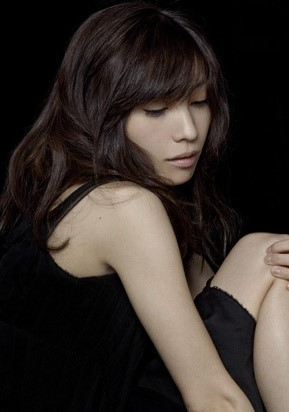
\includegraphics[width=0.7\textwidth]{onitsuka_chihiro.jpg}
%\caption{fig1}
\end{minipage}
}
\subfigure[鬼束千寻]{
\begin{minipage}[t]{0.5\linewidth}
\centering
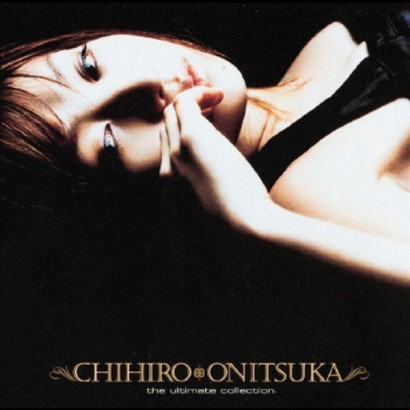
\includegraphics[width=0.7\textwidth]{onitsuka_chihiro_2.jpg}
%\caption{fig1}
\end{minipage}
}
\end{figure}

鬼束千寻是80世代的创作型女歌手,其一直以神秘的形象而著称。2000年,一首《月光》惊艳了整个日本和台湾乐坛,长期霸榜,一度成为热点话题。2002年仅22岁便在武道馆公演成功,未来无可限量。\\
但不幸的是,2003年由于声带问题不得不终止活动,迎来漫长而艰苦的养病生活,甚至一度忧郁症自杀未遂。2004年养好病之后活动再开,人气稳步上升,但是也达不到02年那么石破天惊般的话题度了。\\
豆瓣评千寻的风格为“词曲意境充满着慈悲心与包容力,摆脱了个人而走入人间”。新浪娱乐评其“她的音乐来自内心浅藏的本能,那毫无算计过的曲风,令人深深感动难以忘怀,尤其她总是能建构出诗人一般的词境,拥有贯穿任何世代的魔力,却又充满慈悲的包容力,于是在日本乐团建立起独一无二的鲜明形象”。
\subsubsection*{歌曲推荐}
\begin{enumerate}
\item 月光
\item 茨の海
\end{enumerate}


\subsection{椎名林檎}

\begin{figure}[h]
\centering
 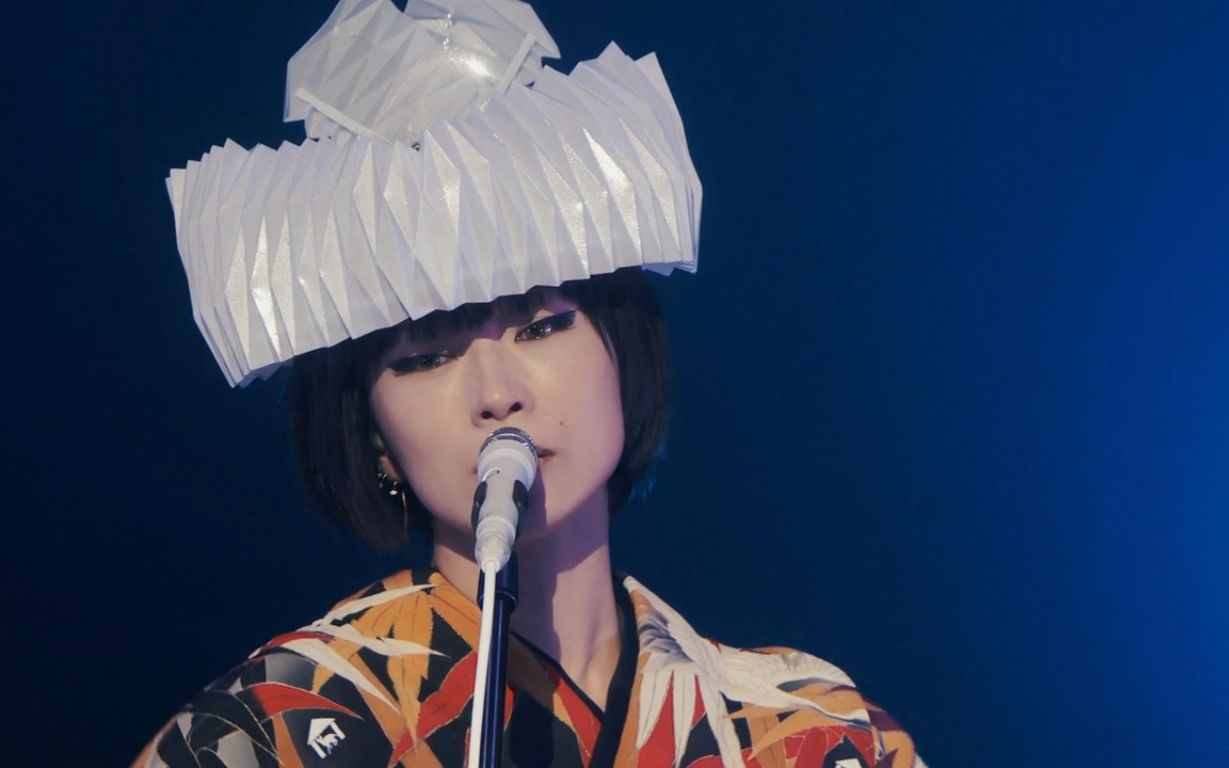
\includegraphics[width=1.0\textwidth]{ringo}
 \caption{椎名林檎}
\end{figure}

椎名林檎人称苹果女王(りんご女王),之所以是女王,大概是由于椎名林檎极富于独特风格的作曲风格。大概在苹果女王眼里,她的歌你想听就听,不想听别bb。所以一旦对上了苹果女王的电波,那么你会有前所未有的“船新感受”,但如果对不上,那就不好意思,大概一秒钟也听不下去了。\\
笔者认识苹果女王是在16年的红白,那一首《長く短い祭》(长短祭)惊艳全场,深深地刺激到了笔者未经世事的耳蜗。从那之后,但凡苹果女王发的新歌都会趋之若鹜,但却难有再次对上电波的了。若不能欣赏,便只剩下噪音。\\
03年,苹果女王成立了后来大名鼎鼎的乐团“东京事变”,并开始了人气飙升之路。直到2012年乐团解散,苹果女王将全身心都投入东京事变的词曲创作,很少有个人活动。乐团解散后,就算林檎开始渐渐淡出音乐圈,但也能做到红白固定登场,足见人气之居高不下。\\
林檎的作曲风格极其多变,其歌词也较为深奥,需要花比较大的力气才能理解她的歌。\\

\subsubsection*{歌曲推荐}
\begin{enumerate}
\item 長く短い祭~ここは地獄か天国か篇~
\item 歌舞伎町の女王
\end{enumerate}


\subsection{KOKIA(吉田亚纪子)}

\begin{figure}[h]
\subfigure[KOKIA]{
\begin{minipage}[t]{0.5\linewidth}
\centering
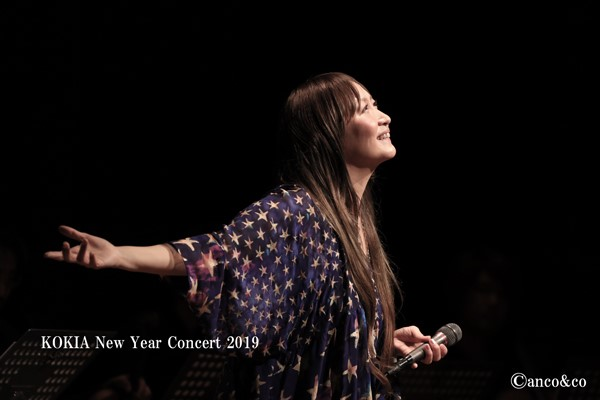
\includegraphics[width=0.7\textwidth]{kokia.jpg}
%\caption{fig1}
\end{minipage}
}
\subfigure[KOKIA]{
\begin{minipage}[t]{0.5\linewidth}
\centering
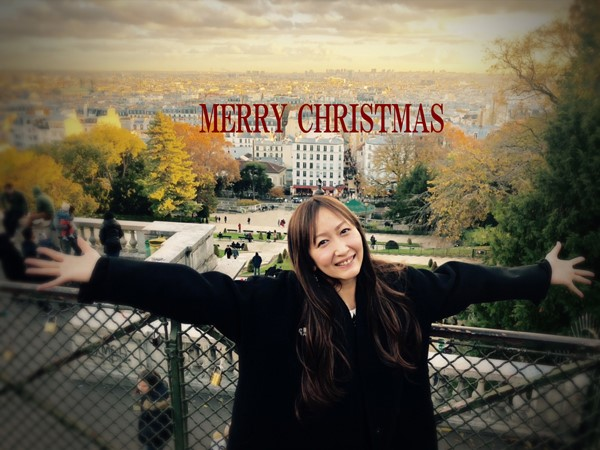
\includegraphics[width=0.7\textwidth]{kokia_2.jpg}
%\caption{fig1}
\end{minipage}
}
\end{figure}

KOKIA原名吉田亚纪子,将亚纪子(AKIKO)倒过来便是KOKIA。亚纪子个人特色鲜明,其声音空灵飘渺,极具感染力。亚纪子初中就读于教会女校,受到大量宗教圣歌的影响,在这时亚纪子便形成了自己音乐风格的雏形。之后高中时期又主攻歌剧,练就一副动人心魄的空灵嗓音。大学时歌姬出道,不久便凭借《ありがとう…》一炮而红。\\
笔者第一次听的亚纪子的歌就是《ありがとう…》,前奏完,开口的一瞬间便如同彗星撞地球,石破天惊的颤音便直接让耳朵怀孕,宛如堕入凡尘的天使在咏唱圣歌,委婉纯洁只可远观不可亵玩。全程跪着听完之后才发现已经站不起来了。\\
早年的亚纪子作曲风格专注于圣歌类古典音乐与民谣,而今愈发多变。但由于近来巡演较多,便也很少发专辑了。\\
亚纪子深受欧美与中国听众喜爱,但相对的在日本的人气却一直并不高。亚纪子与ACG届的合作很多,创作了许多游戏的主题曲,所以在阿宅中人气较高,但在普罗大众中并不闻名。\\


\subsubsection*{歌曲推荐}
\begin{enumerate}
\item ありがとう…
\item EXEC\_ COSMOFLIPS \_.
\item 白雪
\end{enumerate}

\section{偏ACG歌手、唱见}
\subsection{水濑祈}
\subsection{鹿乃}
\subsubsection*{歌曲推荐}
\begin{enumerate}
\item アイロニ
\end{enumerate}
\subsection{小缘}
\subsubsection*{歌曲推荐}
\begin{enumerate}
\item 心做し
\end{enumerate}
\subsection{majico}
\subsubsection*{歌曲推荐}
\begin{enumerate}
\item 君に最後の口づけを
\end{enumerate}

\end{document}